\documentclass[aspectratio=169, 14pt]{beamer}
\usepackage[utf8]{inputenc}
\usepackage[english]{babel}
\usepackage{tipa}
\usepackage{graphicx}
\usepackage{transparent}
\usepackage[ruled, lined, linesnumbered, commentsnumbered]{algorithm2e}
\usepackage{tikz}
\usetikzlibrary{calc,shadows.blur}
\usetikzlibrary{matrix,backgrounds}
\usetikzlibrary{arrows, positioning}
\usetikzlibrary {arrows.meta}
\usetikzlibrary{decorations.pathmorphing, patterns}
\pgfdeclaredecoration{penciline}{initial}{
    \state{initial}[width=+\pgfdecoratedinputsegmentremainingdistance,auto corner on length=1mm,]{
        \pgfpathcurveto%
        {% From
            \pgfqpoint{\pgfdecoratedinputsegmentremainingdistance}
                            {\pgfdecorationsegmentamplitude}
        }
        {%  Control 1
        \pgfmathrand
        \pgfpointadd{\pgfqpoint{\pgfdecoratedinputsegmentremainingdistance}{0pt}}
                        {\pgfqpoint{-\pgfdecorationsegmentaspect\pgfdecoratedinputsegmentremainingdistance}%
                                        {\pgfmathresult\pgfdecorationsegmentamplitude}
                        }
        }
        {%TO 
        \pgfpointadd{\pgfpointdecoratedinputsegmentlast}{\pgfpoint{1pt}{1pt}}
        }
    }
    \state{final}{}
}
\usepackage{minted}
\usepackage{csquotes}
\usepackage{outlines}
\usepackage{booktabs}
\usepackage{hyperref}
\hypersetup{
    colorlinks=true,
    linkcolor=blue,
    filecolor=magenta,      
    urlcolor=cyan,
    }
\urlstyle{same}
\usetheme{metropolis}
\metroset{block=fill}
\usecolortheme{default}
\definecolor{darkmidnightblue}{rgb}{0.0, 0.2, 0.4}
\definecolor{LightGray}{gray}{0.9}


%------------------------------------------------------------
%This block of code defines the information to appear in the
%Title page
\title[Data Structures] %optional
{Data Structures}

\subtitle{Queues and Deques}

\author[CHEN Zhongpu] % (optional)
{CHEN Zhongpu}

\institute[] % (optional)
{
  School of Computing and Artificial Intelligence \\
  \href{mailto:zpchen@swufe.edu.cn}{zpchen@swufe.edu.cn}
}

\date[] % (optional)
{SWUFE, Fall 2022}

%End of title page configuration block
%------------------------------------------------------------


%------------------------------------------------------------
%The next block of commands puts the table of contents at the 
%beginning of each section and highlights the current section:

% \AtBeginSection[]
% {
%   \begin{frame}
%     \frametitle{Table of Contents}
%     \tableofcontents[currentsection]
%   \end{frame}
% }
%------------------------------------------------------------


\begin{document}

%The next statement creates the title page.
\frame{\titlepage}

%---------------------------------------------------------
%This block of code is for the table of contents after
%the title page
% \begin{frame}
% \frametitle{Table of Contents}
% \tableofcontents
% \end{frame}
%--------------------------------------------------------
\begin{frame}[fragile]
    \frametitle{A Small Quiz}
    \begin{itemize}
        \item Why does inserting an element in front of a \texttt{list} cost more time than inserting one at the end of a \texttt{list}?
    \end{itemize}
\begin{itemize}
    \item What does it print?
\end{itemize}
    
\begin{minted}[bgcolor=LightGray,baselinestretch=0.9]{python}
s = Stack()
s.push(1)   
s.push(9)
s.push(8)
print(s.pop())
\end{minted}
\end{frame}

{
    % \usebackgroundtemplate{\transparent{0.3}{\begin{picture}
    %     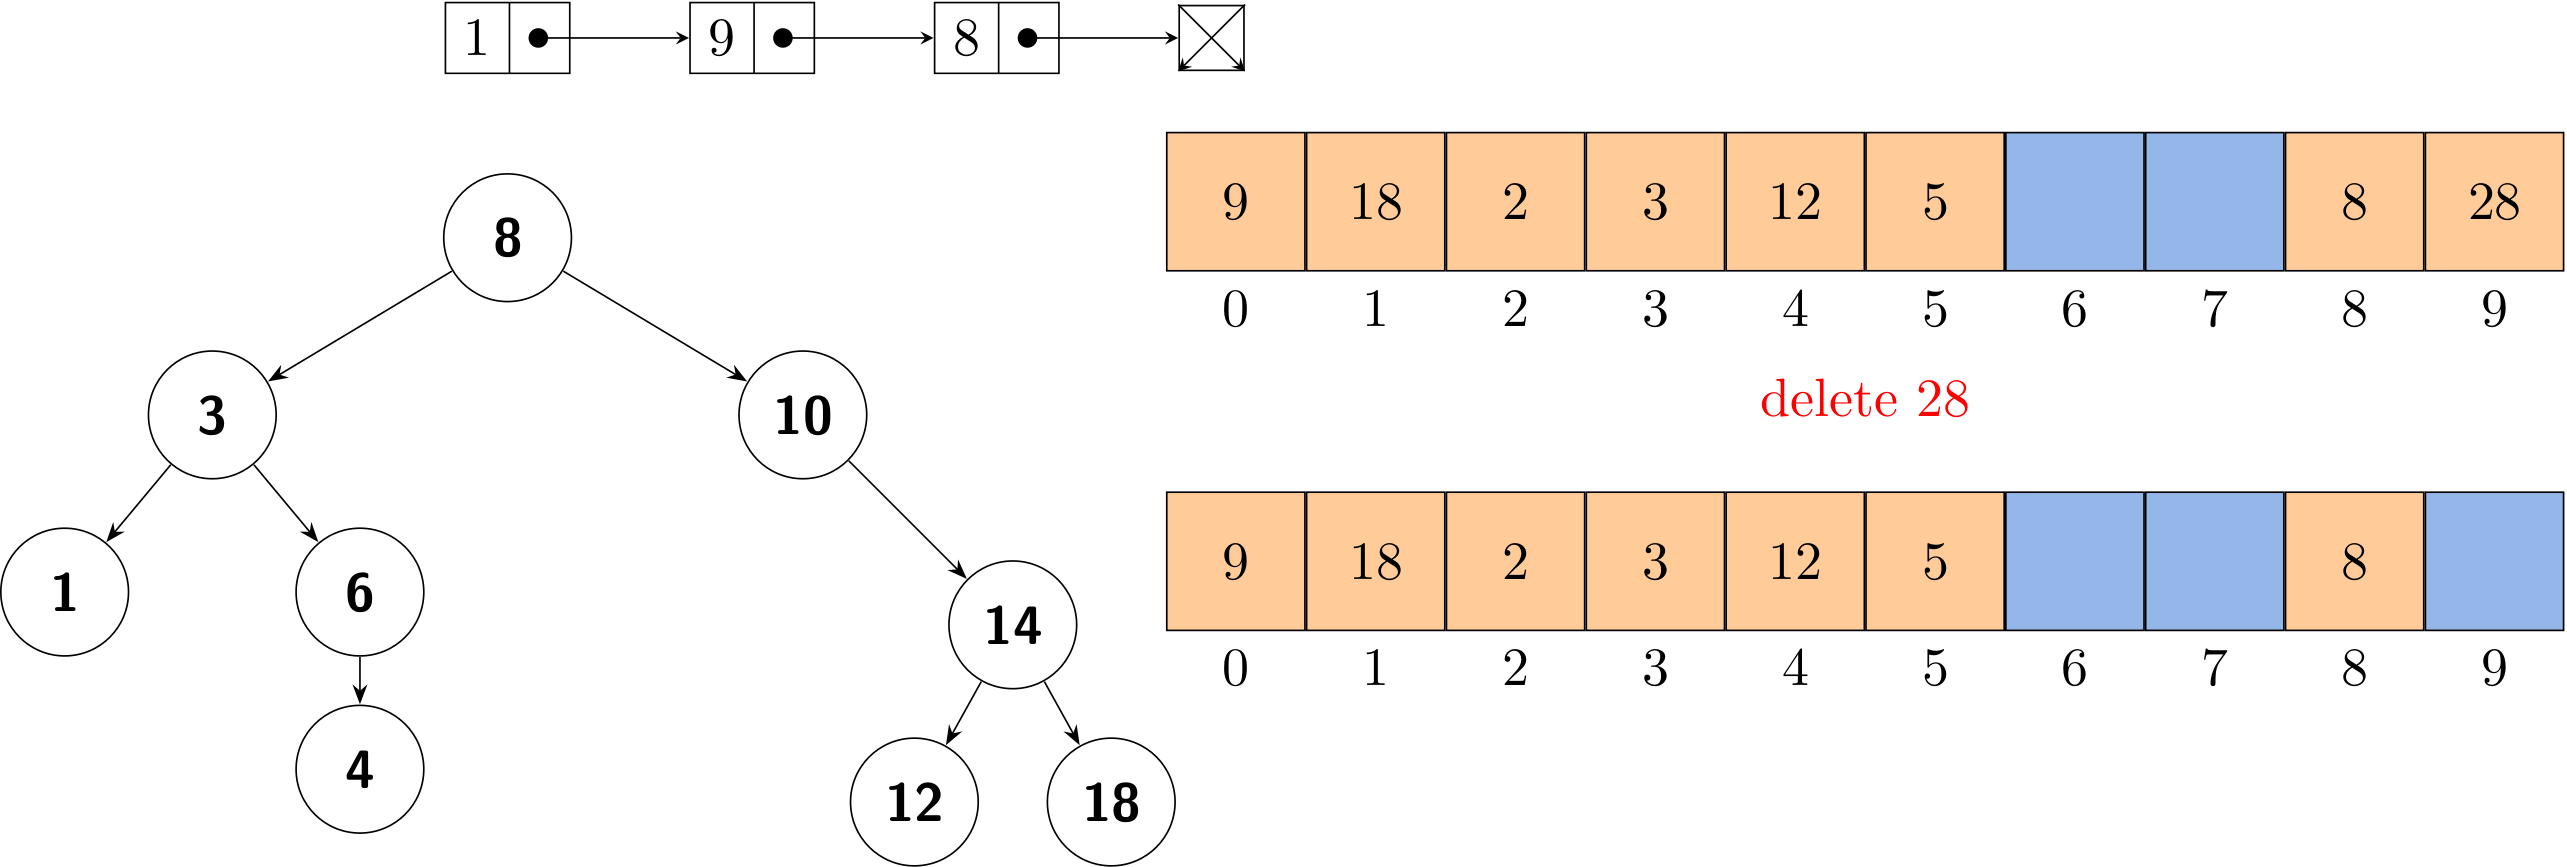
\includegraphics[height=0.7\paperheight]{cover}
    % \end{picture}    
    % }}
\usebackgroundtemplate{
  \tikz[overlay,remember picture] 
  \node[opacity=0.3, at=(current page.south east),anchor=south east, yshift=2cm,xshift=4cm] {
    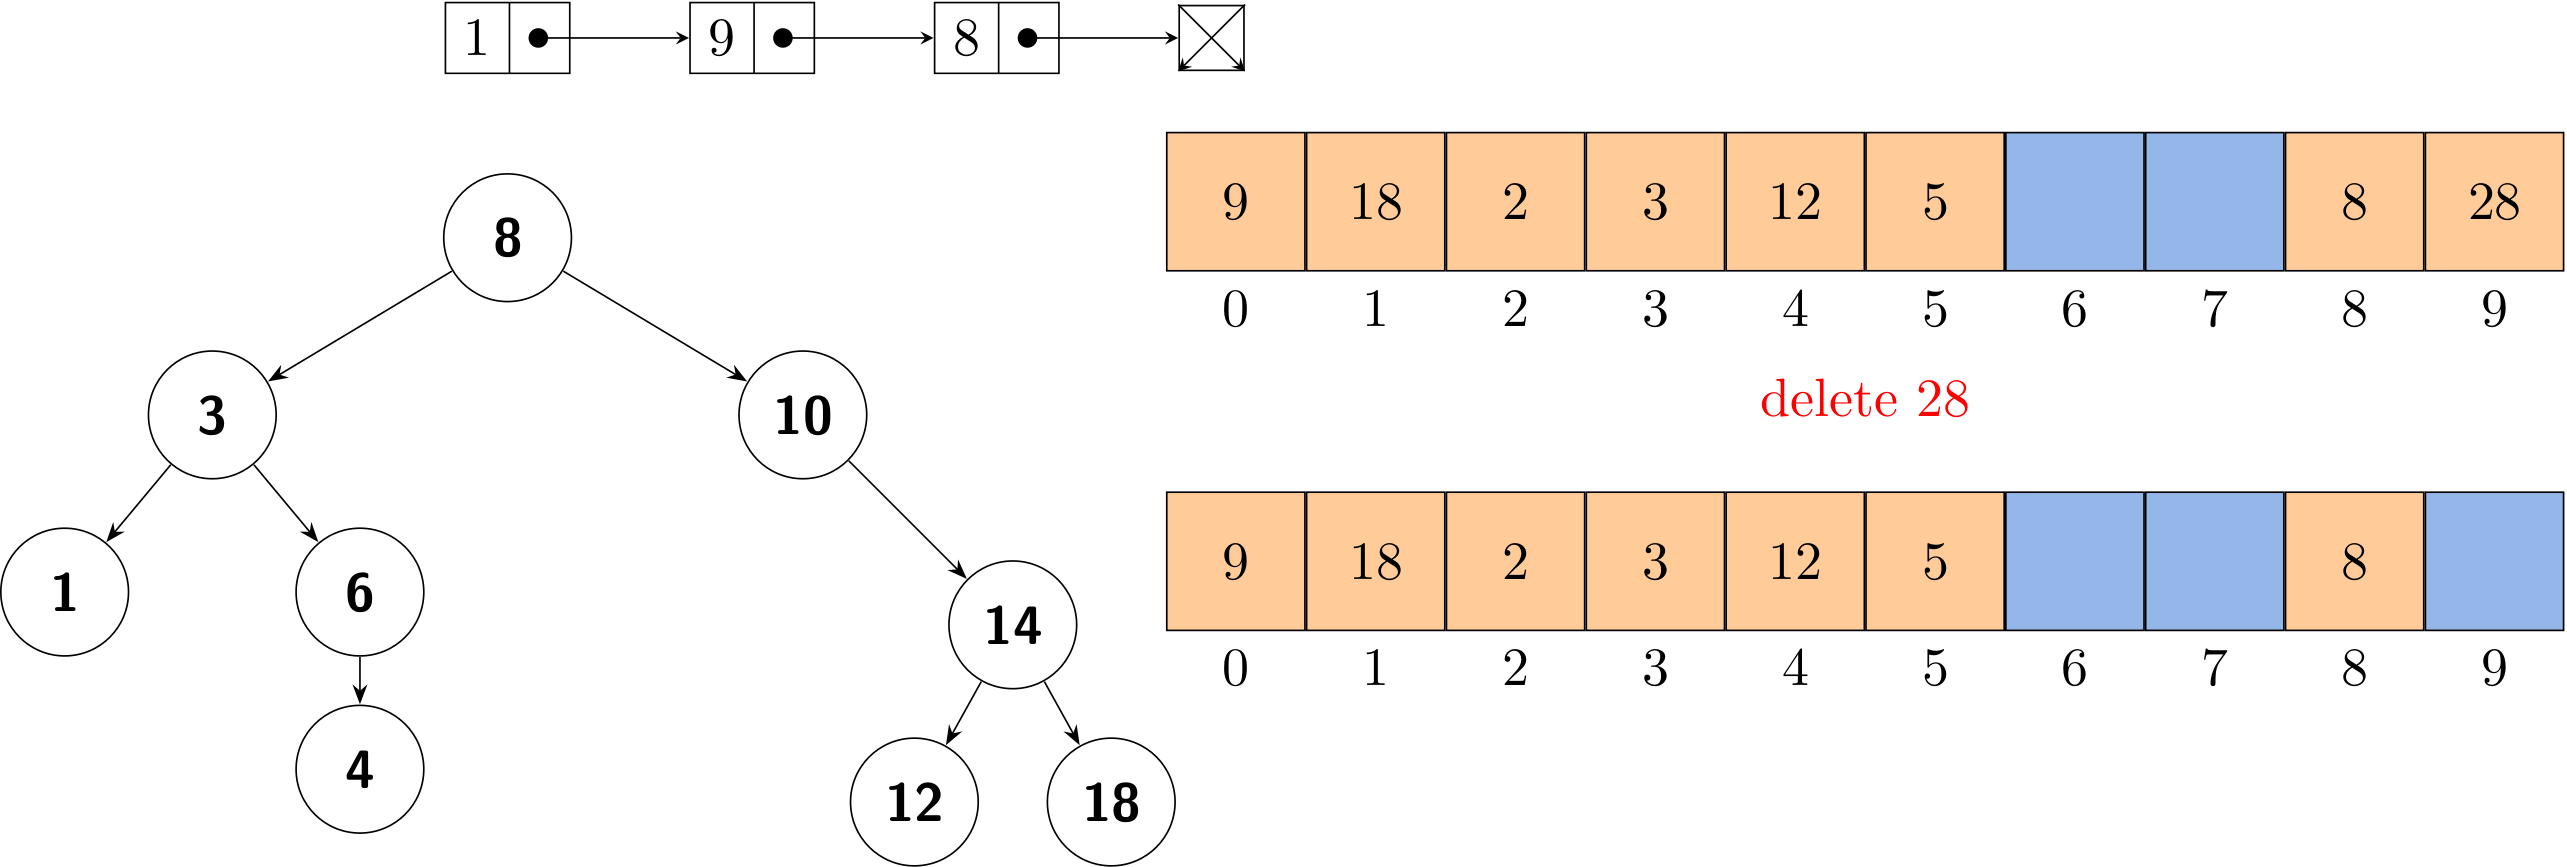
\includegraphics[height=0.6\paperheight]{cover}};
}
    \begin{frame}
        \section{\textcolor{darkmidnightblue}{Queue}}
    \end{frame}
}

\begin{frame}
    % \frametitle{Queue}

   \begin{center}
    
\includegraphics[height=.5\paperheight]{week4/atm}
   \end{center} 
   \begin{quote}
    Queue: a line of people, usually standing or in cars, waiting for something.
    \begin{flushright}
        --- from Cambridge dictionary
    \end{flushright}
\end{quote}
\end{frame}

\begin{frame}
    \frametitle{Queue}

    \begin{exampleblock}{Queue}
        A queue is a collection of objects that are inserted and removed according to the 
        \alert{first-in, first-out (FIFO)} policy.        
    \end{exampleblock}
    \pause
    It supports two basic operations:
    \begin{itemize}
        \item \texttt{enqueue()}: add a new element
        \item \texttt{dequeue()}: remove an element
    \end{itemize}
    Additionally, it also supports other operations such as \texttt{size()}, \texttt{isEmpty()}, and \texttt{peek()}.
\end{frame}

\begin{frame}[fragile]

\begin{columns}
    \column{0.4\textwidth}<1->
        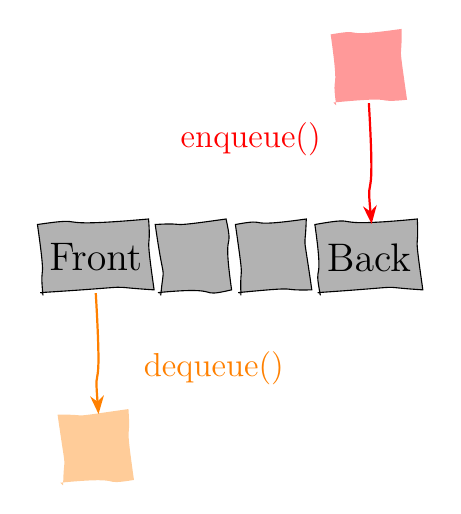
\begin{tikzpicture}[slot/.style={minimum size=0.9cm,rectangle}, data/.style={slot, fill=black!30}, enqueue/.style={slot, fill=red!40}, dequeue/.style={slot, fill=orange!40}, >=Stealth, decoration=penciline]
        \matrix [nodes=draw]
        {
          \node[data, decorate] (n1) {\Large Front}; &
          \node[data, decorate] (n2) {}; &
          \node[data, decorate] (n3) {}; & 
          \node[data, decorate] (n4) {\Large Back}; &
          \\ 
        };
        \node[enqueue, decorate, above=of n4, yshift=0.5cm] (n5) {};
        \draw[->, thick, red, decorate] (n5) -- (n4) node[yshift=1.5cm, xshift=-1.5cm] {\large enqueue()};
        \node[dequeue, decorate, below=of n1, yshift=-0.5cm] (n6) {}; 
        \draw[->, thick, orange, decorate] (n1) -- (n6) node[yshift=1cm, xshift=1.5cm] {\large dequeue()};
    \end{tikzpicture}
    \column{0.6\textwidth}<2->
    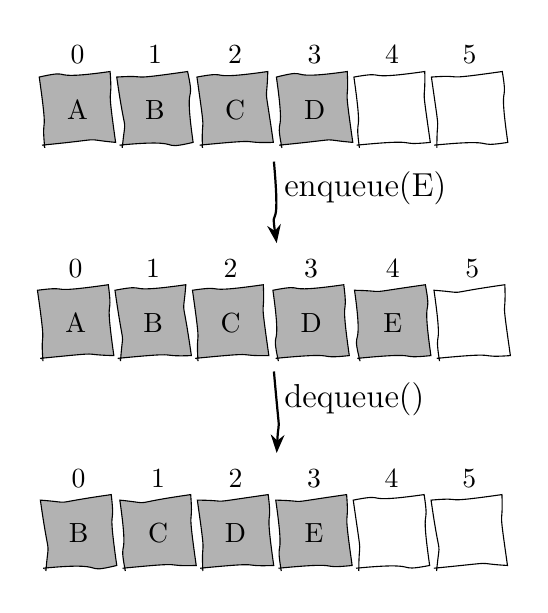
\begin{tikzpicture}[slot/.style={minimum size=0.9cm,rectangle}, data/.style={slot, fill=black!30}, >=Stealth, decoration=penciline]

        \matrix [nodes=draw](before)
        {
          \node[data, decorate, label={0}] (n1) {A}; &
          \node[data, decorate, label={1}] (n2) {B}; &
          \node[data, decorate, label={2}] (n3) {C}; & 
          \node[data, decorate, label={3}] (n4) {D}; &
          \node[slot, decorate, label={4}] (n5) {}; &
          \node[slot, decorate, label={5}] (n6) {}; 
          \\ 
        };
    
        \matrix [nodes=draw, below=of before](after)
        {
          \node[data, decorate, label={0}] (2n1) {A}; &
          \node[data, decorate, label={1}] (2n2) {B}; &
          \node[data, decorate, label={2}] (2n3) {C}; & 
          \node[data, decorate, label={3}] (2n4) {D}; &
          \node[data, decorate, label={4}] (2n5) {E}; &
          \node[slot, decorate, label={5}] (2n6) {}; 
          \\ 
        };
    
        \draw[->, decorate, thick] (before) -- (after) node[right, yshift=1.5cm] {\large enqueue(E)};
    
        \matrix [nodes=draw, below=of after](after2)
        {
          \node[data, decorate, label={0}] (3n1) {B}; &
          \node[data, decorate, label={1}] (3n2) {C}; &
          \node[data, decorate, label={2}] (3n3) {D}; & 
          \node[data, decorate, label={3}] (3n4) {E}; &
          \node[slot, decorate, label={4}] (3n5) {}; &
          \node[slot, decorate, label={5}] (3n6) {}; 
          \\ 
        }; 
    
        \draw[->, decorate, thick] (after) -- (after2) node[right, yshift=1.5cm] {\large dequeue()};    
    \end{tikzpicture}
\end{columns}


\end{frame}

\begin{frame}[fragile]
    \begin{minted}[bgcolor=LightGray,baselinestretch=0.9]{python}
class Queue:
    """A FIFO data structure."""

    def __init__(self):
        self._data = []

    def enqueue(self, item):
        self._data.append(item)

    def dequeue(self):
        if self.is_empty():
            raise NoElement()
        return self._data.pop(0)
    \end{minted}
\end{frame}

\begin{frame}
    \frametitle{Time Complexity}
    \begin{table}
        \caption{Queue's time complexity}
        \begin{tabular}{lr}
          \toprule
          Operation & Complexity\\
          \midrule
          \texttt{enqueue()} & $O(1)$\\
          \texttt{dequeue()} & $O(N)$ \\
          \texttt{size()} & $O(1)$ \\
          \texttt{is\_empty()} & $O(1)$ \\ 
          \bottomrule
        \end{tabular}
    \end{table}    
    Note that the \texttt{dequeue()} is inefficient as it grows linearly with respect to the size of the queue.
\end{frame}

\begin{frame}
    \frametitle{Circular Queue}
A better way is to \textbf{use an array circularly}. Such structure is also known as a \alert{ring buffer} or \alert{circular buffer} in many applications.

\begin{columns}
    \column{0.5\textwidth}
    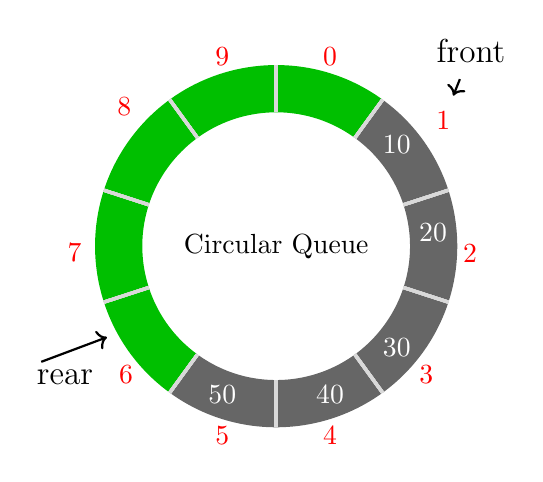
\begin{tikzpicture}
        \colorlet{good}{green!75!black}
        \colorlet{bad}{red}
        \colorlet{neutral}{black!60}
        \colorlet{none}{white}
      
        \node[align=center,text width=3cm]{Circular Queue};
      
        \begin{scope}[line width=6mm,rotate=270]
          \draw[good]          (144:2cm) arc (144:324:2cm);
          \draw[neutral]       (-36:2cm) arc (-36:144:2cm);
      
          \newcount\mycount
          \foreach \angle in {0,72,...,3599}
          {
            \mycount=\angle\relax
            \divide\mycount by 2\relax
            \draw[black!15,very thick] (\the\mycount:17mm) -- (\the\mycount:23mm);
          }
          
          \draw (160:2cm) node[above, red] {0};
    
          \draw (135:3cm) node[below, red] (1) {1};
          \draw (135:3.5cm) node (front) {
            \large front}; 
          \draw [<-, thick] (front) -- (1);
          \draw (130:2cm) node[white] {10};
    
          \draw (100:2.5cm) node[below, red] {2}; 
          \draw (95:2cm) node[white] {20}; 
    
          \draw (60:2.2cm) node[below, red] {3}; 
          \draw (50:2cm) node[white] {30}; 
    
          \draw (20:2cm) node[below, red] {4};
          \draw (20:2cm) node[white] {40};
    
          \draw (-20:2cm) node[below, red] {5};
          \draw (-20:2cm) node[white] {50}; 
    
          \draw (-60:2.2cm) node[below, red] (6) {6};
          \node[below left=of 6, yshift=2cm, xshift=1.5cm] (rear) {\large rear}; 
          \node at (-60:2cm) (6th) {};
          \draw[->, thick] (rear)++ (-0.2,-0.3) -- (6th);
          \draw (-100:2.6cm) node[below, red] {7};
          \draw (-140:3cm) node[below, red] {8}; 
          \draw (-160:2cm) node[above, red] {9};
    
        \end{scope}
    \end{tikzpicture}
    \column{0.5\textwidth}
    \begin{itemize}
        \item \textbf{front}: the pointer to the first item
        \item \textbf{rear}: the pointer to the next available position
    \end{itemize}
\end{columns}

\end{frame}

\begin{frame}
    \begin{columns}
        \column{0.5\textwidth}
        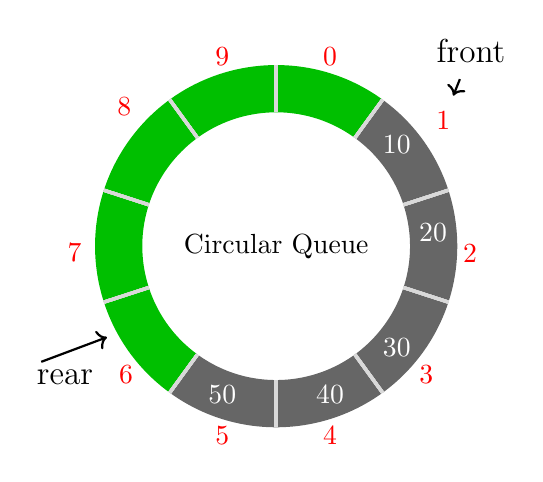
\begin{tikzpicture}
            \colorlet{good}{green!75!black}
            \colorlet{bad}{red}
            \colorlet{neutral}{black!60}
            \colorlet{none}{white}
          
            \node[align=center,text width=3cm]{Circular Queue};
          
            \begin{scope}[line width=6mm,rotate=270]
              \draw[good]          (144:2cm) arc (144:324:2cm);
              \draw[neutral]       (-36:2cm) arc (-36:144:2cm);
          
              \newcount\mycount
              \foreach \angle in {0,72,...,3599}
              {
                \mycount=\angle\relax
                \divide\mycount by 2\relax
                \draw[black!15,very thick] (\the\mycount:17mm) -- (\the\mycount:23mm);
              }
              
              \draw (160:2cm) node[above, red] {0};
        
              \draw (135:3cm) node[below, red] (1) {1};
              \draw (135:3.5cm) node (front) {
                \large front}; 
              \draw [<-, thick] (front) -- (1);
              \draw (130:2cm) node[white] {10};
        
              \draw (100:2.5cm) node[below, red] {2}; 
              \draw (95:2cm) node[white] {20}; 
        
              \draw (60:2.2cm) node[below, red] {3}; 
              \draw (50:2cm) node[white] {30}; 
        
              \draw (20:2cm) node[below, red] {4};
              \draw (20:2cm) node[white] {40};
        
              \draw (-20:2cm) node[below, red] {5};
              \draw (-20:2cm) node[white] {50}; 
        
              \draw (-60:2.2cm) node[below, red] (6) {6};
              \node[below left=of 6, yshift=2cm, xshift=1.5cm] (rear) {\large rear}; 
              \node at (-60:2cm) (6th) {};
              \draw[->, thick] (rear)++ (-0.2,-0.3) -- (6th);
              \draw (-100:2.6cm) node[below, red] {7};
              \draw (-140:3cm) node[below, red] {8}; 
              \draw (-160:2cm) node[above, red] {9};
        
            \end{scope}
        \end{tikzpicture}
        \column{0.5\textwidth}
        \begin{itemize}
            \item \texttt{enqueue()}: update \alert{rear} to next one in the clock-wise
            \item \texttt{dequeue()}: update \alert{front} to next one in the clock-wise
        \end{itemize}

        \large \[front + size = rear\]
    \end{columns}
\end{frame}

\begin{frame}
    \begin{columns}
        \column{0.4\textwidth}
        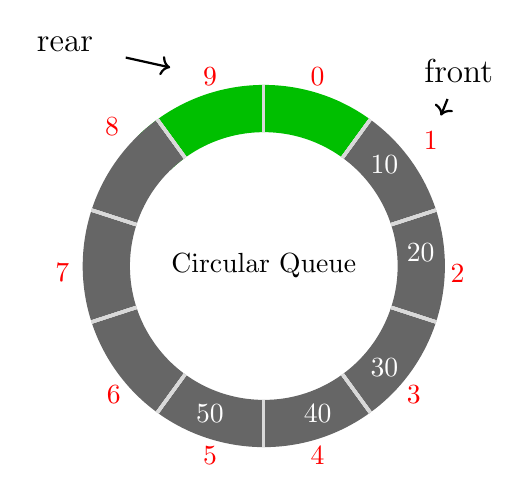
\begin{tikzpicture}
            \colorlet{good}{green!75!black}
            \colorlet{bad}{red}
            \colorlet{neutral}{black!60}
            \colorlet{none}{white}
          
            \node[align=center,text width=3cm]{Circular Queue};
          
            \begin{scope}[line width=6mm,rotate=270]
              \draw[good]          (144:2cm) arc (144:224:2cm);
              \draw[neutral]       (-144:2cm) arc (-144:144:2cm);
          
              \newcount\mycount
              \foreach \angle in {0,72,...,3599}
              {
                \mycount=\angle\relax
                \divide\mycount by 2\relax
                \draw[black!15,very thick] (\the\mycount:17mm) -- (\the\mycount:23mm);
              }
              
              \draw (160:2cm) node[above, red] {0};
        
              \draw (135:3cm) node[below, red] (1) {1};
              \draw (135:3.5cm) node (front) {
                \large front}; 
              \draw [<-, thick] (front) -- (1);
              \draw (130:2cm) node[white] {10};
        
              \draw (100:2.5cm) node[below, red] {2}; 
              \draw (95:2cm) node[white] {20}; 
        
              \draw (60:2.2cm) node[below, red] {3}; 
              \draw (50:2cm) node[white] {30}; 
        
              \draw (20:2cm) node[below, red] {4};
              \draw (20:2cm) node[white] {40};
        
              \draw (-20:2cm) node[below, red] {5};
              \draw (-20:2cm) node[white] {50}; 
        
              \draw (-60:2.2cm) node[below, red] (6) {6};
              \draw (-100:2.6cm) node[below, red] {7};
              \draw (-140:3cm) node[below, red] {8}; 
              \draw (-160:2cm) node[above, red] (9) {9};
              \node[xshift=-1.5cm] at (-160:3cm) (rear) {\large rear};
              \draw [->, thick] (rear) -- (9); 
            \end{scope}
        \end{tikzpicture}
        \column{0.55\textwidth}
        What will \alert{rear} become after calling one more \texttt{enqueue()}?
\pause

\begin{block}{Modular}
    $front \gets (front + 1) \ mod \ capacity$
    $rear \gets (front + size) \ mod \ capacity$
\end{block}

       
    \end{columns} 
\end{frame}

\begin{frame}[fragile]
    \begin{columns}
        \column{0.4\textwidth}<1-> 
        \begin{table}
            \caption{Time complexity}
            \begin{tabular}{lr}
              \toprule
              Operation & Complexity\\
              \midrule
              \texttt{enqueue()} & $O(1)$\\
              \texttt{dequeue()} & $O(1)$ \\
              \texttt{size()} & $O(1)$ \\
              \texttt{is\_empty()} & $O(1)$ \\ 
              \bottomrule
            \end{tabular}
        \end{table} 
        \column{0.6\textwidth}<2->
        \begin{minted}[bgcolor=LightGray,baselinestretch=0.9]{python}
class CircularQueue:
    def __init__(self):
        self._data = [None]*10
        self._size = 0
        self._front = 0
        \end{minted}
    \end{columns}
\end{frame}

\begin{frame}[fragile]
    \begin{minted}[baselinestretch=1, bgcolor=LightGray]{python}
def enqueue(self, item):
    avail = (self._front + self._size) % len(self._data)
    self._data[avail] = item
    self._size += 1

def dequeue(self):
    if self.is_empty():
        raise NoElement()
    answer = self._data[self._front]
    self._data[self._front] = None
    self._front = (self._front + 1) % len(self._data)
    self._size -= 1
    return answer
    \end{minted} 
\end{frame}
\begin{frame}[fragile]
    \frametitle{Resizing}
    As for a circular array, we need deal with the \textbf{resizing} for either enlarging or shrinking.

    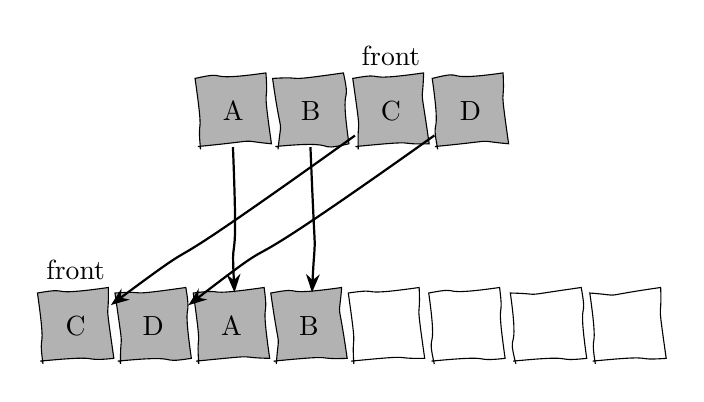
\begin{tikzpicture}[slot/.style={minimum size=0.9cm,rectangle}, data/.style={slot, fill=black!30}, enqueue/.style={slot, fill=red!40}, dequeue/.style={slot, fill=orange!40}, >=Stealth, decoration=penciline]
        \matrix [nodes=draw](table1)
        {
          \node[data, decorate] (a1) {A}; &
          \node[data, decorate] (b1) {B}; &
          \node[data, decorate, label={front}] (c1) {C}; & 
          \node[data, decorate] (d1) {D}; &
          \\ 
        };
        
        \matrix [nodes=draw, below=of table1](table2)
        {
          \node[data, decorate, label={front}] (c2) {C}; &
          \node[data, decorate] (d2) {D}; &
          \node[data, decorate] (a2) {A}; & 
          \node[data, decorate] (b2) {B}; &
          \node[slot, decorate]  {}; &
          \node[slot, decorate]  {}; &
          \node[slot, decorate]  {}; &
          \node[slot, decorate]  {}; &
          \\ 
        };

        \draw[->, thick, decorate] (c1) -- (c2);
        \draw[->, thick, decorate] (d1) -- (d2);
        \draw[->, thick, decorate] (a1) -- (a2);
        \draw[->, thick, decorate] (b1) -- (b2);
    \end{tikzpicture}
\end{frame}

\begin{frame}[fragile]
    \begin{minted}[bgcolor=LightGray]{python}
def _resize(self, capacity):
    assert capacity > self.size()
    old = self._data
    self._data = [None] * capacity
    walk = self._front
    for i in range(self._size):
        self._data[i] = old[walk]
        walk = (1 + walk) % len(old)
    self._front = 0
    \end{minted} 
\end{frame}

\section{\textcolor{darkmidnightblue}{Deque}}

\begin{frame}[fragile]
    \frametitle{Deque}
Double ended queue, or \alert{deque}. It is often pronounced \emph{deck} to avoid confusion.

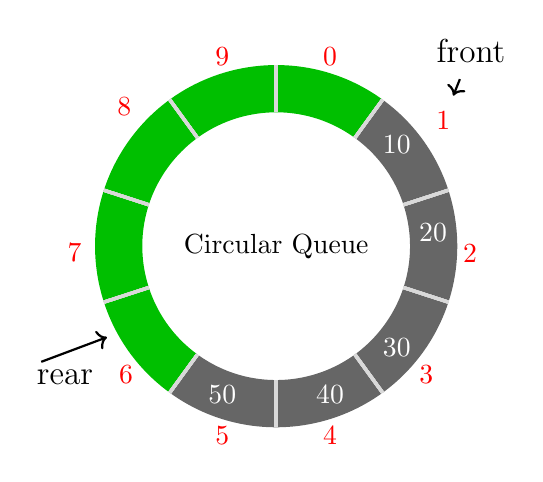
\begin{tikzpicture}
    \colorlet{good}{green!75!black}
    \colorlet{bad}{red}
    \colorlet{neutral}{black!60}
    \colorlet{none}{white}
  
    \node[align=center,text width=3cm]{Circular Queue};
  
    \begin{scope}[line width=6mm,rotate=270]
      \draw[good]          (144:2cm) arc (144:324:2cm);
      \draw[neutral]       (-36:2cm) arc (-36:144:2cm);
  
      \newcount\mycount
      \foreach \angle in {0,72,...,3599}
      {
        \mycount=\angle\relax
        \divide\mycount by 2\relax
        \draw[black!15,very thick] (\the\mycount:17mm) -- (\the\mycount:23mm);
      }
      
      \draw (160:2cm) node[above, red] {0};

      \draw (135:3cm) node[below, red] (1) {1};
      \draw (135:3.5cm) node (front) {
        \large front}; 
      \draw [<-, thick] (front) -- (1);
      \draw (130:2cm) node[white] {10};

      \draw (100:2.5cm) node[below, red] {2}; 
      \draw (95:2cm) node[white] {20}; 

      \draw (60:2.2cm) node[below, red] {3}; 
      \draw (50:2cm) node[white] {30}; 

      \draw (20:2cm) node[below, red] {4};
      \draw (20:2cm) node[white] {40};

      \draw (-20:2cm) node[below, red] {5};
      \draw (-20:2cm) node[white] {50}; 

      \draw (-60:2.2cm) node[below, red] (6) {6};
      \node[below left=of 6, yshift=2cm, xshift=1.5cm] (rear) {\large rear}; 
      \node at (-60:2cm) (6th) {};
      \draw[->, thick] (rear)++ (-0.2,-0.3) -- (6th);
      \draw (-100:2.6cm) node[below, red] {7};
      \draw (-140:3cm) node[below, red] {8}; 
      \draw (-160:2cm) node[above, red] {9};

    \end{scope}
\end{tikzpicture}    
\end{frame}

\begin{frame}[fragile]
    \frametitle{Deque In Python}

    Luckily, \href{https://docs.python.org/3/library/collections.html}{collections.deque} has been designed in Python, which have fast appends and pops from both ends.

    \begin{minted}[bgcolor=LightGray]{python}
from collections import deque
q = deque(['structures', 'is'])
q.append('fun') # add_last
q.append('!') # add_last
q.appendleft('data') # add_first
q.pop() # delete_last
print(q)
q.popleft() # delete_first
print(q)
    \end{minted} 

\end{frame}

\begin{frame}[fragile]
    \frametitle{Deque In Java}
    Java is shipped with the \href{https://docs.oracle.com/en/java/javase/11/docs/api/java.base/java/util/Deque.html}{Deque} interface as well as many useful implementing classes, including \href{https://docs.oracle.com/en/java/javase/11/docs/api/java.base/java/util/ArrayDeque.html}{ArrayDeque}, \href{https://docs.oracle.com/en/java/javase/11/docs/api/java.base/java/util/LinkedList.html}{LinkedList}.    
    \begin{minted}[bgcolor=LightGray]{java}
Deque<String> deque = new ArrayDeque<>();
deque.offerLast("structures");
deque.offerLast("is");
deque.offerFirst("data");
deque.offerLast("fun");
    \end{minted} 
\end{frame}

{\setbeamercolor{palette primary}{fg=black, bg=yellow}
\begin{frame}[standout]
The \alert{deque} provides complete and consistent set of both LIFO stack operations and FIFO queue operations.
\end{frame}
}

\begin{frame}[fragile]
    \frametitle{LeetCode 933. Number of Recent Calls}
\href{https://leetcode.com/problems/number-of-recent-calls/}{933. Number of Recent Calls}
\pause
\begin{minted}[bgcolor=LightGray, baselinestretch=1, fontsize=\footnotesize]{python}
from collections import deque


class RecentCounter:
    def __init__(self):
        self.data = deque()

    def ping(self, t: int) -> int:
        while len(self.data) > 0 and (t - 3000) > self.data[0]:
            self.data.popleft()
        self.data.append(t)
        return len(self.data)
\end{minted}
\end{frame}

\begin{frame}
\section{\textcolor{darkmidnightblue}{Conclusion}}
    \begin{enumerate}
        \item Queue, deque
        \item Circular array
        \item Language built-in libraries
    \end{enumerate}
\end{frame}
\begin{frame}
    \frametitle{Homework 2}
\begin{enumerate}
    \item Exercise 11, Chapter 2. (10 marks)
    \item Please elaborate how to use two \texttt{stacks} as a \texttt{queue}; how about the time complexity?  (5 marks).
\end{enumerate}
\end{frame}
\end{document}